% !TeX root = ./../../main.tex
% Sfera Blocha i interferencja jednokubitowa (podrozdział 2.1, rys. fig:tb01:bloch).
% (a) sfera Blocha (plik tb01_bloch_sphere.tex),
% (b) obwód H - P(phi) - H z pomiarem,
% (c) prawdopodobieństwa wyników w funkcji fazy lokalnej:
%     p(0) = (1 + cos phi)/2, p(1) = (1 - cos phi)/2 oraz p(0) = (1 + v cos phi)/2 dla v = 0,6 (stłumione koherencje).
\begin{subfigure}[c]{0.36\textwidth}
  \centering
  % !TeX root = ./../../main.tex
% Sfera Blocha (podrozdział 2.1, rys. fig:tb01:bloch, panel a; wstawiana przez tb01_interference.tex).
% Rzut prostokątny: azymut obserwatora 25 stopni, elewacja 20 stopni.
% Wektory jednostkowe osi x, y, z w rzucie: (-0.423,-0.310), (0.906,-0.145), (0,0.940).
% Widoczna część równika: t od -65 do 115 stopni.
\begin{tikzpicture}[
    scale=1.5,
    x={(-0.423cm,-0.310cm)}, y={(0.906cm,-0.145cm)}, z={(0cm,0.940cm)},
    axis/.style={-{Stealth[length=2mm]}, thin},
    aux/.style={densely dashed, thin, gray},
    every node/.style={font=\small}
  ]
  % kontur sfery (w rzucie prostokątnym jest okręgiem)
  \draw[thin] (0,0,0) ++(0cm,0cm) circle[radius=1cm];
  % równik: część niewidoczna i widoczna
  \draw[aux] plot[domain=115:295, samples=60, variable=\t] ({cos(\t)}, {sin(\t)}, 0);
  \draw[thin] plot[domain=-65:115, samples=60, variable=\t] ({cos(\t)}, {sin(\t)}, 0);
  % osie
  \draw[axis] (0,0,0) -- (1.35,0,0) node[below left=-1pt] {$x$};
  \draw[axis] (0,0,0) -- (0,1.3,0) node[right] {$y$};
  \draw[axis] (0,0,0) -- (0,0,1.3) node[above] {$z$};
  \draw[aux] (0,0,0) -- (-1,0,0);
  \draw[aux] (0,-1,0) -- (0,0,0);
  \draw[aux] (0,0,-1) -- (0,0,0);
  % stany bazowe i stany na równiku
  \fill (0,0,1) circle[radius=0.7pt] node[above right=-1pt and 1pt] {$\ket{0}$};
  \fill (0,0,-1) circle[radius=0.7pt] node[below] {$\ket{1}$};
  \fill (1,0,0) circle[radius=0.7pt] node[below right=0pt and 1pt] {$\ket{+}$};
  \fill (0,1,0) circle[radius=0.7pt] node[above=3pt] {$\ket{+\mathrm{i}}$};
  % stan |psi> dla theta = 50 stopni, phi = 60 stopni
  \coordinate (P) at ({sin(50)*cos(60)}, {sin(50)*sin(60)}, {cos(50)});
  \coordinate (Q) at ({sin(50)*cos(60)}, {sin(50)*sin(60)}, 0);
  \draw[aux, black] (0,0,0) -- (Q) -- (P);
  \draw[-{Stealth[length=2.2mm]}, thick] (0,0,0) -- (P) node[above right=-1pt and -1pt] {$\ket{\psi}$};
  \fill (P) circle[radius=0.8pt];
  % kąt theta (od osi z do wektora stanu)
  \draw[thin] plot[domain=0:50, samples=20, variable=\s] ({0.3*sin(\s)*cos(60)}, {0.3*sin(\s)*sin(60)}, {0.3*cos(\s)});
  \node at ({0.42*sin(25)*cos(60)}, {0.42*sin(25)*sin(60)}, {0.42*cos(25)}) {$\theta$};
  % kąt phi (od osi x do rzutu wektora stanu na płaszczyznę równika)
  \draw[thin] plot[domain=0:60, samples=20, variable=\s] ({0.35*cos(\s)}, {0.35*sin(\s)}, 0);
  \node at ({0.5*cos(30)}, {0.5*sin(30)}, 0) {$\varphi$};
\end{tikzpicture}

  \caption{}\label{fig:tb01:bloch:sphere}
\end{subfigure}\hfill
\begin{minipage}[c]{0.6\textwidth}
  \begin{subfigure}{\linewidth}
    \centering
    \begin{quantikz}[column sep=0.25cm]
      \lstick{$\ket{0}$} & \gate{\mathrm{H}} & \gate{\mathrm{P}(\varphi)} & \gate{\mathrm{H}} & \meter{}
    \end{quantikz}
    \caption{}\label{fig:tb01:interference:circuit}
  \end{subfigure}

  \medskip
  \begin{subfigure}{\linewidth}
    \centering
    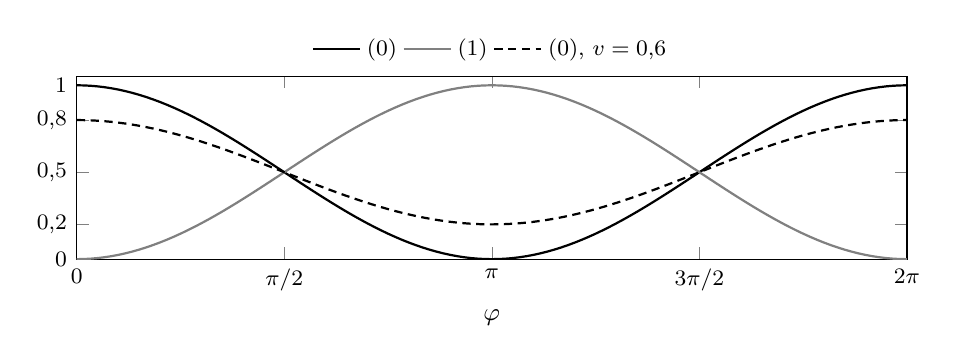
\begin{tikzpicture}
      \begin{axis}[
          width=\linewidth, height=3.9cm,
          xmin=0, xmax=6.2832, ymin=0, ymax=1.05,
          xtick={0,1.5708,3.1416,4.7124,6.2832},
          xticklabels={$0$,$\pi/2$,$\pi$,$3\pi/2$,$2\pi$},
          ytick={0,0.2,0.5,0.8,1},
          yticklabels={$0$,$0{,}2$,$0{,}5$,$0{,}8$,$1$},
          xlabel={$\varphi$},
          legend style={font=\footnotesize, at={(0.5,1.03)}, anchor=south, draw=none, legend columns=3},
          tick label style={font=\footnotesize}, label style={font=\small},
          samples=121, domain=0:6.2832,
        ]
        \addplot[thick, black] {(1+cos(deg(x)))/2};
        \addlegendentry{$\prob(\ket{0})$}
        \addplot[thick, gray] {(1-cos(deg(x)))/2};
        \addlegendentry{$\prob(\ket{1})$}
        \addplot[thick, black, densely dashed] {(1+0.6*cos(deg(x)))/2};
        \addlegendentry{$\prob(\ket{0})$, $v=0{,}6$}
      \end{axis}
    \end{tikzpicture}
    \caption{}\label{fig:tb01:interference:plot}
  \end{subfigure}
\end{minipage}
